\documentclass[fleqn]{report}
\usepackage{graphicx} % om PostScript plaatje in te lassen
\usepackage{here}     % voor geforceerde plaatsing figuren
\usepackage{amsmath}
\textwidth=17.0cm
\textheight=22.0cm
\topmargin=-1cm
\oddsidemargin=-0.3cm
\evensidemargin=-0.3cm

%packages
\usepackage{amsmath}
\usepackage{cite}
\usepackage[toc,page]{appendix}
\usepackage{fancyvrb}
\usepackage{tikz}
\usepackage{multicol}
\usepackage{framed}
\usepackage{pgfplots}
\usepackage{fixltx2e}
\usepackage{subfigure}
\usepackage{lscape}
\usepackage{enumitem}
\usepackage{filecontents}

%tikz labraries
\usetikzlibrary{matrix}
\usetikzlibrary{decorations.pathreplacing}
\usetikzlibrary{positioning}
\usetikzlibrary{calc}
\usetikzlibrary{shapes,arrows, chains}
\usetikzlibrary{intersections}
\usetikzlibrary{decorations.markings}
\usetikzlibrary{calc,intersections}
 \usetikzlibrary{svg.path}
 \usetikzlibrary{patterns}
\usepackage{xcolor}
%\usetikzlibrary{decorations.pathreplacing,bending}

%extra instellingen
\newlist{aims}{enumerate}{1}
\setlist[aims,1]{
  label={*},
  leftmargin=*,
  align=left,
  labelsep=2mm,
}

\newlist{aims2}{enumerate}{1}
\setlist[aims2,1]{
  label={},
  leftmargin=0pt,
  align=left,
  labelsep=4mm,
}

\newlist{aims3}{enumerate}{1}
\setlist[aims3,1]{
  label={-},
  leftmargin=2cm,
  align=left,
  labelsep=0.4mm,
}

\usepackage{pgfplots}

\begin{document}


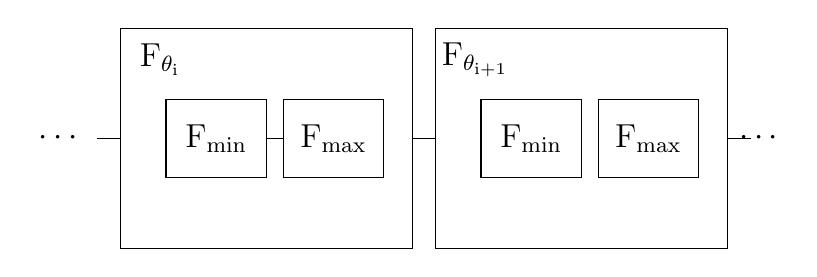
\begin{tikzpicture}
\footnotesize

% used shapes
\tikzstyle{block} = [rectangle, draw, node distance = 0.2cm, text width=1cm, text centered, minimum height=1cm]
\tikzstyle{diamond_thing} = [diamond, draw, node distance = 0.5cm, text centered, minimum height=1cm]
\tikzstyle{blokje} = [rectangle, draw, rounded corners = 5pt, node distance = 0.5cm, text width=2cm, text centered, minimum height=0.5cm,fill=purple!20]
\tikzstyle{blockrounded} = [rectangle, draw, rounded corners = 5pt, node distance = 1cm, fill=yellow!20, text width=3cm, text centered, minimum height=0.5cm]
\tikzstyle{blockroundedred} = [rectangle, draw, rounded corners = 5pt, node distance = 1cm, fill=red!20, text width=3cm, text centered, minimum height=0.5cm]

\large

\draw (-3,0) -- (-2.7,0);
\draw (-2.7,-1.4) rectangle (1,1.4);

\node at (-2.2, 1) {$\mathrm{F}_{\mathrm{\theta_i}}$};

\node [block] (max)  {$\mathrm{F}_{\mathrm{max}}$};

\node [block, left = of max] (min)  {$\mathrm{F}_{\mathrm{min}}$};

\draw (min) -- (max);

\begin{scope}[shift={(4,0)}]
 \draw (-3,0) -- (-2.7,0);
\draw (-2.7,-1.4) rectangle (1,1.4);

\node at (-2.2, 1) {$\mathrm{F}_{\mathrm{\theta_{i+1}}}$};

\node [block] (max)  {$\mathrm{F}_{\mathrm{max}}$};

\node [block, left = of max] (min)  {$\mathrm{F}_{\mathrm{min}}$};

\end{scope}



\draw (5,0) -- (5.3,0);

\node at (-3.5, 0) {$\mathbf{\cdots}$};
\node at (5.4, 0) {$\mathbf{\cdots}$};

\end{tikzpicture}





\end{document}